
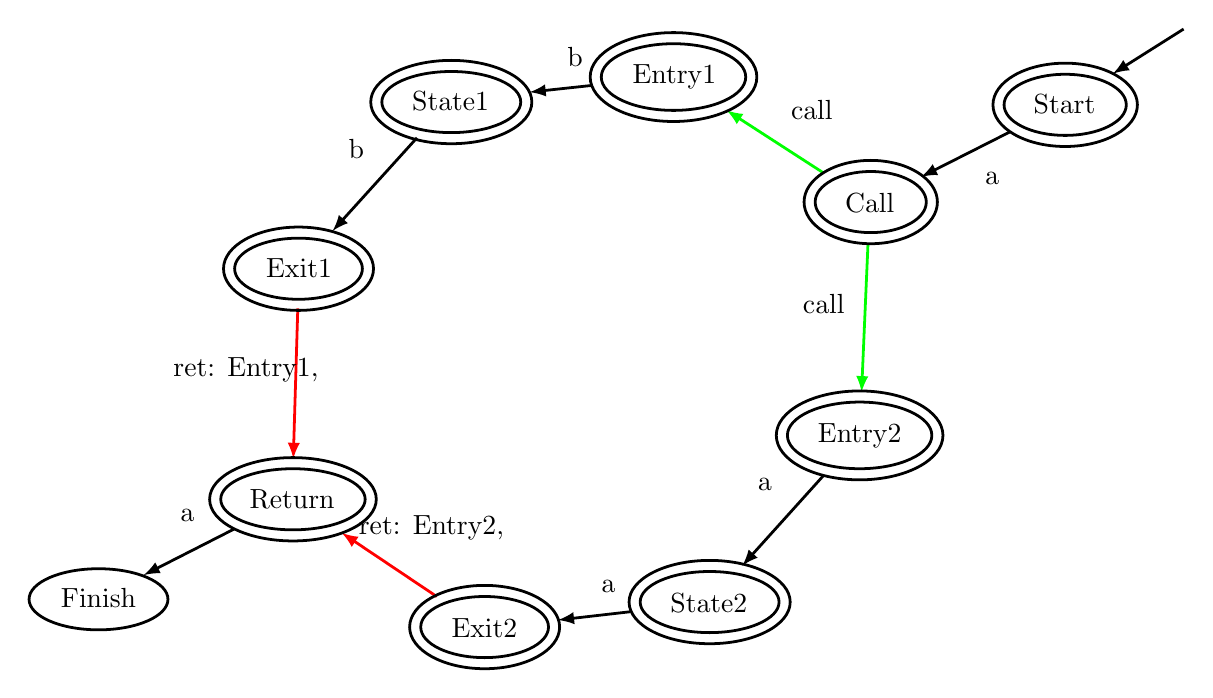
\begin{tikzpicture}[>=latex,line join=bevel,]
  \pgfsetlinewidth{1bp}
%%
\pgfsetcolor{black}
  % Edge: Exit2 -> Return
  \pgfsetcolor{red}
  \draw [->] (147.8bp,26.972bp) .. controls (139.99bp,32.207bp) and (130.57bp,38.522bp)  .. (113.56bp,49.923bp);
  \definecolor{strokecol}{rgb}{0.0,0.0,0.0};
  \pgfsetstrokecolor{strokecol}
  \draw (145.85bp,51.654bp) node {ret: Entry2, };
  % Edge: Call -> Entry1
  \pgfsetcolor{green}
  \draw [->] (286.98bp,179.5bp) .. controls (279.12bp,184.58bp) and (269.53bp,190.77bp)  .. (252.09bp,202.05bp);
  \definecolor{strokecol}{rgb}{0.0,0.0,0.0};
  \pgfsetstrokecolor{strokecol}
  \draw (282.81bp,202.01bp) node {call};
  % Edge: State2 -> Exit2
  \draw [->] (217.47bp,21.52bp) .. controls (212.31bp,20.929bp) and (206.86bp,20.305bp)  .. (191.4bp,18.534bp);
  \draw (209.49bp,30.605bp) node {a};
  % Edge: Exit1 -> Return
  \pgfsetcolor{red}
  \draw [->] (97.741bp,130.71bp) .. controls (97.378bp,118.6bp) and (96.854bp,101.07bp)  .. (96.121bp,76.536bp);
  \definecolor{strokecol}{rgb}{0.0,0.0,0.0};
  \pgfsetstrokecolor{strokecol}
  \draw (79.083bp,108.72bp) node {ret: Entry1, };
  % Edge: State1 -> Exit1
  \draw [->] (140.63bp,192.12bp) .. controls (133.71bp,184.47bp) and (124.87bp,174.72bp)  .. (110.25bp,158.56bp);
  \draw (118.84bp,188.1bp) node {b};
  % Edge: Start -> Call
  \draw [->] (354.23bp,194.32bp) .. controls (347.09bp,190.7bp) and (338.87bp,186.54bp)  .. (322.11bp,178.06bp);
  \draw (347.69bp,177.48bp) node {a};
  % Edge: Call -> Entry2
  \pgfsetcolor{green}
  \draw [->] (303.02bp,154.14bp) .. controls (302.5bp,142.19bp) and (301.76bp,125bp)  .. (300.7bp,100.55bp);
  \definecolor{strokecol}{rgb}{0.0,0.0,0.0};
  \pgfsetstrokecolor{strokecol}
  \draw (287.08bp,132.44bp) node {call};
  % Edge: Entry2 -> State2
  \draw [->] (287.16bp,70.726bp) .. controls (280.42bp,63.237bp) and (272.02bp,53.922bp)  .. (257.77bp,38.107bp);
  \draw (265.86bp,67.183bp) node {a};
  % Edge: Entry1 -> State1
  \draw [->] (203.77bp,211bp) .. controls (199.74bp,210.57bp) and (195.55bp,210.12bp)  .. (181.2bp,208.57bp);
  \draw (197.58bp,221.34bp) node {b};
  % Edge: Return -> Finish
  \draw [->] (74.776bp,51.264bp) .. controls (67.366bp,47.49bp) and (58.949bp,43.203bp)  .. (42.241bp,34.695bp);
  \draw (57.997bp,56.265bp) node {a};
  % Edge: Start__precursor__ -> Start
  \draw [->] (416.63bp,231.28bp) .. controls (411.26bp,227.89bp) and (405.37bp,224.17bp)  .. (391.15bp,215.19bp);
  % Node: Entry2
\begin{scope}
  \definecolor{strokecol}{rgb}{0.0,0.0,0.0};
  \pgfsetstrokecolor{strokecol}
  \draw (300bp,85bp) ellipse (26bp and 12bp);
  \draw (300bp,85bp) ellipse (30bp and 16bp);
  \draw (300.03bp,85.004bp) node {Entry2};
\end{scope}
  % Node: Entry1
\begin{scope}
  \definecolor{strokecol}{rgb}{0.0,0.0,0.0};
  \pgfsetstrokecolor{strokecol}
  \draw (233bp,214bp) ellipse (26bp and 12bp);
  \draw (233bp,214bp) ellipse (30bp and 16bp);
  \draw (233.31bp,214.19bp) node {Entry1};
\end{scope}
  % Node: Exit1
\begin{scope}
  \definecolor{strokecol}{rgb}{0.0,0.0,0.0};
  \pgfsetstrokecolor{strokecol}
  \draw (98bp,145bp) ellipse (23bp and 11bp);
  \draw (98bp,145bp) ellipse (27bp and 15bp);
  \draw (98.175bp,145.22bp) node {Exit1};
\end{scope}
  % Node: State2
\begin{scope}
  \definecolor{strokecol}{rgb}{0.0,0.0,0.0};
  \pgfsetstrokecolor{strokecol}
  \draw (246bp,25bp) ellipse (25bp and 11bp);
  \draw (246bp,25bp) ellipse (29bp and 15bp);
  \draw (245.74bp,24.758bp) node {State2};
\end{scope}
  % Node: Exit2
\begin{scope}
  \definecolor{strokecol}{rgb}{0.0,0.0,0.0};
  \pgfsetstrokecolor{strokecol}
  \draw (165bp,16bp) ellipse (23bp and 11bp);
  \draw (165bp,16bp) ellipse (27bp and 15bp);
  \draw (164.91bp,15.5bp) node {Exit2};
\end{scope}
  % Node: Start
\begin{scope}
  \definecolor{strokecol}{rgb}{0.0,0.0,0.0};
  \pgfsetstrokecolor{strokecol}
  \draw (374bp,204bp) ellipse (22bp and 11bp);
  \draw (374bp,204bp) ellipse (26bp and 15bp);
  \draw (373.76bp,204.2bp) node {Start};
\end{scope}
  % Node: State1
\begin{scope}
  \definecolor{strokecol}{rgb}{0.0,0.0,0.0};
  \pgfsetstrokecolor{strokecol}
  \draw (153bp,205bp) ellipse (25bp and 11bp);
  \draw (153bp,205bp) ellipse (29bp and 15bp);
  \draw (152.74bp,205.5bp) node {State1};
\end{scope}
  % Node: Finish
\begin{scope}
  \definecolor{strokecol}{rgb}{0.0,0.0,0.0};
  \pgfsetstrokecolor{strokecol}
  \draw (26bp,26bp) ellipse (25bp and 11bp);
  \draw (26bp,26.423bp) node {Finish};
\end{scope}
  % Node: Call
\begin{scope}
  \definecolor{strokecol}{rgb}{0.0,0.0,0.0};
  \pgfsetstrokecolor{strokecol}
  \draw (304bp,169bp) ellipse (20bp and 11bp);
  \draw (304bp,169bp) ellipse (24bp and 15bp);
  \draw (303.65bp,168.72bp) node {Call};
\end{scope}
  % Node: Return
\begin{scope}
  \definecolor{strokecol}{rgb}{0.0,0.0,0.0};
  \pgfsetstrokecolor{strokecol}
  \draw (96bp,62bp) ellipse (26bp and 11bp);
  \draw (96bp,62bp) ellipse (30bp and 15bp);
  \draw (95.683bp,61.911bp) node {Return};
\end{scope}
%
\end{tikzpicture}
